\section{Дополнительные примеры распределений $d^2\sigma/(dx\,dQ^2)$}
\label{sec:examples_extrapolated_region}

Для полноты картины на рис.~(\ref{Pp3}) и~(\ref{Pp6}) приведены примеры дважды дифференциальных нормированных сечений $\frac{1}{\sigma(E_\nu)}\frac{d^2\sigma(E_\nu,x,Q^2)}{dx\,dQ^2}$ для энергий нейтрино $E_\nu = 1$~ТэВ и $1$~ПэВ. 
Рассмотренные распределения иллюстрируют, как с ростом энергии нейтрино максимум функции постепенно смещается в область меньших значений переменной Бьёркена~$x$, что отражает возрастающее значение вклада малых $x$ в полное сечение. 

\begin{figure}[!h]
\centering
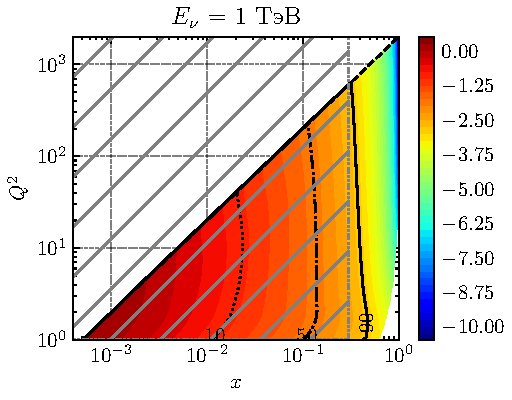
\includegraphics[width=0.8\linewidth]{images/NuProp/cdfxq2_cc_proton_CT18ZNNLO_14_1000.pdf}
\caption{Кумулятивное нормированное сечение $F_{\sigma}(x,Q^2)$ в зависимости от переменных Бьёркена~$x$ и $Q^2$ при энергии нейтрино $E_{\nu} = 1$~ТэВ. Использованы партонные распределения \texttt{CT10nlo}.}
\label{Pp3}
\end{figure}

\begin{figure}[!h]
\centering
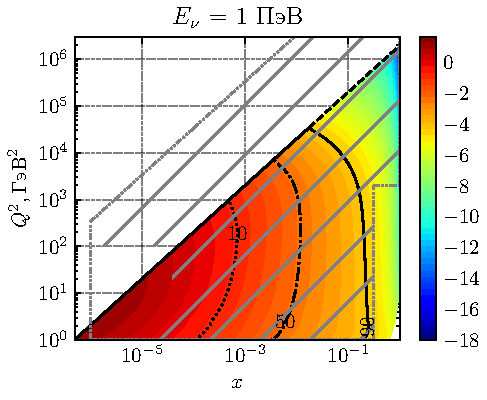
\includegraphics[width=0.8\linewidth]{images/NuProp/cdfxq2_cc_proton_CT18ZNNLO_14_1000000.pdf}
\caption{Кумулятивное нормированное сечение $F_{\sigma}(x,Q^2)$ в зависимости от переменных Бьёркена~$x$ и $Q^2$ при энергии нейтрино $E_{\nu} = 1$~ПэВ. Использованы партонные распределения \texttt{CT10nlo}.}
\label{Pp6}
\end{figure}

Сравнение рисунков показывает, что при увеличении энергии нейтрино до ПэВ-уровня область значимых вкладов смещается в диапазон $x \lesssim 10^{-5}$, подтверждая выводы раздела~\ref{sec:dis_reliability} о растущем влиянии малых~$x$ на формирование полного сечения.
